\chapter{Client-Side e Server-Side}\label{cap:cap_02}

\begin{flushright}
	\textit{
		Viva como se fosse morrer amanhã. \\ Aprenda como se fosse viver para sempre.
	} \\
	\textbf{Mahatma Gandhi}
\end{flushright}

Client-Side (Lado do cliente) e Server-Side (lado do servidor) são dois termos importantes envolvidos no desenvolvimento de software e web. As duas categorias de desenvolvimento têm muitas diferenças, incluindo diferentes propósitos e linguagens de programação. Assim, como nosso objetivo é trabalhar com o desenvolvimento de software, é importante que possamos  entender o desenvolvimento tanto do lado do cliente quanto a do lado do servidor. Assim, nossa jornada se inicia entendendo um dos lados, o do servidor, a qual fará parte do nosso curso durante nossos próximo três semestre. 

\section{O que é desenvolvimento do lado do cliente?}

O desenvolvimento do lado do cliente é uma categoria de desenvolvimento que envolve programas executados em um cliente ou dispositivo do usuário. Os(as) desenvolvedores(as) do lado do cliente se concentram em criar a parte de um sistema com a qual o usuário pode interagir. Às vezes, o desenvolvimento do lado do cliente também é chamado, erroneamente, de desenvolvimento \textbf{front-end}, pois se concentra na parte ``frontal'' de um aplicativo que os usuários podem ver. Os(as) desenvolvedores(as) do lado do cliente concluem uma variedade de tarefas, incluindo:

\begin{itemize}[leftmargin=1.7cm]
	\setlength\itemsep{0em}
	\item Criação de layouts de sites
	\item Projetando interfaces de usuário
	\item Adicionando validação de formulário
	\item Adicionando elementos visuais como cores e fontes
\end{itemize}

Pessoas que desenvolvem para o lado do cliente se preocupam com a experiência do usuário e usam linguagens de programação específicas. Algumas linguagens comuns do lado do cliente incluem:

\begin{itemize}[leftmargin=1.7cm]
	\setlength\itemsep{0em}
	\item  O \textbf{HTML}, que significa\textit{ Hypertext Markup Language}, é uma linguagem de marcação padrão para desenvolvimento web. HTML constrói a estrutura de um site o renderiza em um navegador.
	
	\item O \textbf{CSS}, que significa \textbf{Cascading Style Sheets}, é uma linguagem de design que os(as) desenvolvedores(as) podem usar para adicionar elementos de design visual a um site codificado em HTML. Os desenvolvedores podem usar CSS para tornar seus sites visualmente atraentes nos dispositivos dos usuários.
	
	\item Já o \textbf{JavaScript} é uma linguagem de programação que os(as) desenvolvedores(as) podem usar para desenvolvimento web, aplicações web e outros propósitos. Os\textbf{} desenvolvedores\textbf{} podem usar \textbf{JavaScript} para tornar os sites dinâmicos e interativos. 
\end{itemize}

Contudo, nos últimos anos, JavaScript se tornou uma linguagem que também pode ser usado do lado do servidor dando ao desenvolvedor(a) maior alcance com o conhecimento adquirido. Contudo, mesmo sendo a mesma linguagem, o objetivo acaba diferindo, por isso, vamos entender melhor como usar o JavaScript do lado do servidor. 

\section{O que é desenvolvimento do lado do servidor?}

O desenvolvimento do lado do servidor é um categoria de desenvolvimento que envolve programas executados em um servidor. Os(as) desenvolvedores(as) do lado do servidor se concentram no desenvolvimento nos bastidores, e o desenvolvimento do lado do servidor também é conhecido, e nesse caso acertadamente, como desenvolvimento ``back-end''. Esse categoria de programação é importante porque os navegadores da Web, ou clientes, interagem com os servidores da Web para recuperar informações. 

\begin{figure}[H]
	\centering
	\caption{Client-Side e Server-Side}
	\frame{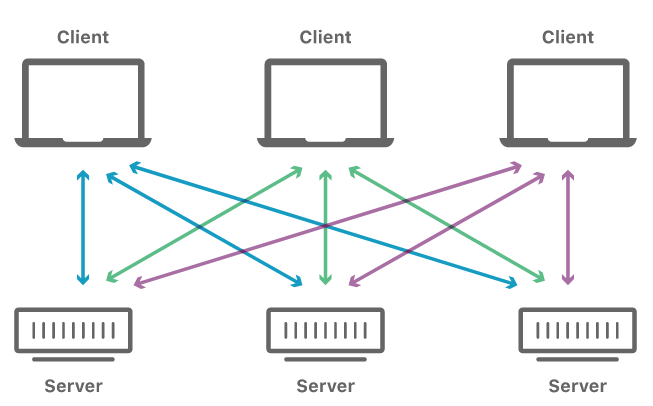
\includegraphics[scale=0.4]{imagens/csss.png}}
	\legend{\textbf{Fonte}: \url{https://bityli.com/jwImTW}}
\end{figure}

As tarefas comuns do lado do servidor incluem:

\begin{itemize}[leftmargin=1.7cm]
	\setlength\itemsep{0em}
	\item Codificando sites dinâmicos
	\item Desenvolvendo aplicações web
	\item Conectando sites a bancos de dados
\end{itemize}

Desenvolvedores(as) de software, administradores(as) de banco de dados e desenvolvedores(as) da Web normalmente usam o desenvolvimento do lado do servidor. Os desenvolvedores do lado do servidor podem usar muitas linguagens de programação diferentes, tais como \textbf{PHP}, \textbf{Java}, \textbf{SQL} e também \textbf{JavaScript} a qual será a linguagem base que usaremos no decorrer do curso.

\section{Lado do cliente vs. lado do servidor}

Lado do cliente e lado do servidor são termos que indicam como e onde o código é executado. Alguns desenvolvedores, chamados desenvolvedores \textbf{full-stack}, sabem como usar o desenvolvimento do lado do cliente e do lado do servidor, pois ambos são importantes para o funcionamento de sites e aplicativos. No entanto, existem algumas diferenças importantes entre o desenvolvimento do lado do cliente e do lado do servidor. Algumas das principais diferenças entre os dois tipos de desenvolvimento incluem:

\subsection{Onde o código é executado?}

Uma grande diferença entre o desenvolvimento do lado do cliente e do lado do servidor é onde o código é executado. No desenvolvimento do lado do cliente, o código é executado no dispositivo do cliente ou do usuário. No entanto, no desenvolvimento do lado do servidor, o código é executado por meio de um servidor. É por isso que o desenvolvimento do lado do cliente também é chamado de front-end e o desenvolvimento do lado do cliente também é back-end.

\subsection{Como é executado?}

A maneira como os códigos são executados é outra diferença entre o desenvolvimento do lado do cliente e do lado do servidor. No código do lado do cliente, o código são simplesmente executados em um dispositivo, muitas vezes em um navegador com pouco ou nenhum acesso à memória do computador. Já do lado do servidor, no entanto, são executados em um servidor web com total acesso à memória do computador.

\subsection{Quais as Finalidades?}

O desenvolvimento do lado do cliente e do lado do servidor também têm propósitos diferentes. O principal objetivo do desenvolvimento do lado do cliente é criar efeitos visuais de sites, incluindo layouts, interfaces de usuário, validação de formulários e outros elementos visuais. O desenvolvimento do lado do servidor, no entanto, concentra-se mais no conteúdo real de uma página da Web e conclui tarefas como interagir com bancos de dados e recuperar informações de um servidor da Web.

\section{Protocolo HTTP}

Um protocolo é um sistema de regras que define como os dados são trafegados dentro ou entre computadores. Comunicações entre dispositivos requer que estes concordem com o formato do dado que estiver sendo trafegado. O conjunto de regras que define esse formato é chamado protocolo.

Podemos representar um protocolo como um meio de comunicação comum a dois indivíduos que não são falantes do mesmo idioma. Assim, uma das maneiras para que a comunicação aconteça e que ambos falem um idioma comum, como, por exemplo, o inglês. Clientes e servidores se comunicam trocando mensagens individuais. As mensagens enviadas pelo cliente, geralmente um navegador da Web, são chamadas de solicitações (requests), ou também requisições, e as mensagens enviadas pelo servidor como resposta são chamadas de respostas (responses).

\begin{figure}[H]
	\centering
	\caption{Analogia Protocolo}
	\frame{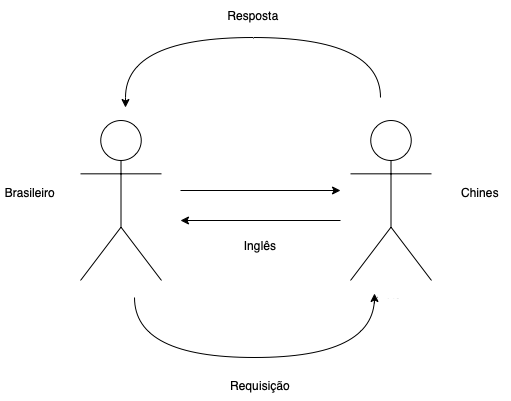
\includegraphics[scale=0.4]{imagens/protocolo.png}}
	\legend{Fonte: O autor}
	\label{fig:protocolo}
\end{figure}

Assim, o HTTP (\textit{Hypertext Transfer Protocol}) segue a mesma dinâmica. O HTTP é um protocolo que permite a obtenção de recursos, como documentos HTML. É a base de qualquer troca de dados na Web e um protocolo cliente-servidor, o que significa que as requisições são iniciadas pelo destinatário, geralmente um navegador da Web. Um documento completo é reconstruído a partir dos diferentes sub-documentos obtidos, como, por exemplo texto, descrição do layout, imagens, vídeos, scripts e muito mais.

\subsection{Métodos de requisição HTTP}

O protocolo HTTP define um conjunto de métodos de requisição responsáveis por indicar a ação a ser executada para um dado recurso. Embora esses métodos possam ser descritos como substantivos, eles também são comumente referenciados como \textit{HTTP Verb}s (Verbos HTTP). O HTTP implementa vários verbos, porém, os mais usados são:

\begin{itemize}[leftmargin=1.7cm]
	\setlength\itemsep{0em}
	\item \textbf{GET}: O método GET solicita a representação de um recurso específico. Requisições utilizando o método GET devem retornar apenas dados.
	\item \textbf{POST}: O método POST é utilizado para submeter uma entidade a um recurso específico, frequentemente causando uma mudança no estado do recurso ou efeitos colaterais no servidor.
	\item \textbf{PUT}: O método PUT substitui todas as atuais representações do recurso de destino pela carga de dados da requisição.
	\item \textbf{DELETE}: O método DELETE remove um recurso específico.
\end{itemize}

\section{Exercícios de fixação}

\begin{enumerate}[leftmargin=1.7cm]
	\setlength\itemsep{0em}
	\item Qual a diferença entre ``Client-Side (lado do cliente) e Server-Side (Lado do servidor)"?
	\item O que é um protocolo e, por que ele é usado na comunicação?
	\item Explique o que é um Verbo HTTP e como eles são utilizados na comunicação.
	\item O JavaScript é uma linguagem Client-Side ou Server-Side? Explique sua resposta.
\end{enumerate}